\documentclass{beamer}
\mode<presentation>
{
  \usetheme[height=40pt]{ScarletHannover} %UNL-Sbaush, MyHannover, BlueHannover, ScarletHannover, Lart
  \useinnertheme[shadow=true]{rounded}
  %\useoutertheme{shadow}  
  
   \usefonttheme{professionalfonts}
  %\usefonttheme{structureitalicserif,structuresmallcapsserif,professionalfonts,serif,structurebold,}
   
   %\usecolortheme{sbaushOUTER} % ---> OUTER
   %\usecolortheme{sbaushINNER} % ---> INNER
   %\usecolortheme{fly}    % ---> COMPLETE
 
%\usecolortheme{default,structure,sidebartab,albatross,dove,fly,seagull,crane,beetle}

%\INNER --> usecolortheme{lily,orchid,rose,}
%\OUTER --> usecolortheme{whale,seahorse,dolphin,}

\setbeamertemplate{navigation symbols}{}
  \setbeamercovered{transparent}
}
\usepackage[italian]{babel}
\usepackage[utf8]{inputenc}
\usepackage{times}
\usepackage[T1]{fontenc}
\usepackage{graphicx}
\usepackage{epsfig}
%\usepackage{beamerouterthemeleo}
%\usepackage{algorithmic}
%\usepackage{algorithm}
%%%%%%%%%%%%%%%
% Definitions %
%%%%%%%%%%%%%%%



%\newcommand{\g}[1]{\alert{#1}}

\institute[Università degli studi di Firenze, Facoltà di Ingegneria] % (optional, but mostly needed)
{
\begin{minipage}[t]{0.4\textwidth}
 \textbf{Docente:} \\ \professor \\
\textbf{Assistenti:} \\ \firstassistant \\  \secondassistant
\end{minipage} 
\hfill
\begin{minipage}[t]{0.4\textwidth}
\begin{flushright}
\textbf{Autori:} \\ \firstauthor \\ \secondauthor \\ \thirdauthor
\end{flushright}
\end{minipage}
}


%\title[Mesh-AP NMS]{Mesh-AP Network Management System}

\title[Analisi Immagini e Video] {Kalman e ConDensation in \textit{video-tracking}}

\subtitle{Sviluppo e comparazione dei due algoritmi per il tracciamento di oggetti su video}

\author[N. Martorana\\I. Masi\\M. Meoni\\ \hrulefill]{Presentazione Elaborato\\ \textsc{ Analisi Immagini e Video}}


\date[Presentazione elaborato] % (optional, should be abbreviation of conference name)
{
   18 Maggio 2007
}


%%%%%%%%%%%%%%%%%%%%%%%%%%%%%%%%%%%%%%%%%%

\begin{document}
\def\firstauthor{Nicola Martorana}
\def\secondauthor{Iacopo Masi}
\def\thirdauthor{Marco Meoni}
\def\coursenumber{ARC}
\def\class{Relazione di Analisi Immagini e Video}
\def\title{Comparazione di Kalman e ConDensation in video-tracking}
\def\semester{2006/2007}
\def\instructor{P. Crescenzi}
\def\date{Maggio 2007}
\def\professor{Prof. Pietro Pala}
\def\firstassistant{Ing. Walter Nunziati}
\def\secondassistant{Ing. Andrew D. Bagdanov}
%%%%%%%%%%%%%%%%%%%%%%%%%%%%%%%%%%%%%%%%%
\frame{\setbeamercolor{titlelike}{bg=UNL@Scarlet,fg=UNL@Cream}
\vspace{-10pt}
\begin{center}
\begin{scriptsize}
	\textsc{Università degli studi di Firenze}
\end{scriptsize}\\ 
\begin{tiny}
	Facoltà di Ingegneria - Corso di laurea specialistica in \textsc{Ingegneria Informatica}
\vspace{-20pt}
\end{tiny}
\end{center}

\titlepage
 }
%%%%%%%%%%%%%%%%%%%%%%%%%%%%%%%%%%%%%%%%%%
\section{Outline}

\frame{\frametitle{Outline}
\begin{itemize}
\item Obiettivi dell'elaborato
\item Metodi di tracking basati su modelli
\begin{itemize}
 \item Kalman Filter
\item ConDensation Filter
\end{itemize}
\item Implementazione dei modelli
\item Sviluppo del Software
\begin{itemize}
 \item Librerie utilizzate
\item Control-flow del programma
\end{itemize}
\item Risultati
\begin{itemize}
 \item Primo video: movies12.mjpeg
\item Secondo video: tappetonomod.avi
\item Terzo video: singlecar.avi
\end{itemize}
\end{itemize}
}
%%%%%%%%%%%%%%%%%%%%%%%%%%%%%%%%%%%%%%%%%%
\section{Obiettivi}
\frame{\frametitle{Obiettivi dell'elaborato}
\begin{itemize}
\item Video-tracking: localizzazione oggetti in movimento su stream video
\begin{itemize}
\item Utilizzato approccio di tracking basato su modelli\end{itemize}
\item Approfondimento dei due metodi più importanti
\begin{itemize}
\item Filtro di Kalman (Anni '50)
\item ConDensation (Anni '90)\end{itemize}
\item Realizzazione software C++ (OpenCV based) per il confronto\end{itemize}
\begin{block}{}
 Confronto tracking basato su Kalman con tracking basato su ConDensation
\end{block}



}
%%%%%%%%%%%%%%%%%%%%%%%%%%%%%%%%%%%%%%%%%%
\section{Tracking}
\frame{\frametitle{Kalman Filter}

Obiettivo: stimare lo stato $x \in \Re^n$ di un processo a tempo discreto governato dalla seguente equazione alle differenze
\begin{equation*}
 x_k=Ax_{k-1}+Bu_{k-1}+w_{k-1}
\end{equation*}  


 L'osservazione (al tempo $k$) dello stato reale $x_k$ è effettuata tramite il vettore della misura $z \in \Re^m$ 


\begin{equation*}
z_k=Hx_k+v_k
\end{equation*}

\begin{figure}[hb]
\centering
	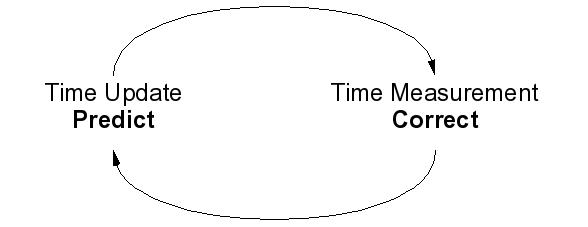
\includegraphics[scale=0.25]{../relazione/figure/PredCorr.jpg}
\caption{\textit{Il ciclio di calcolo del filtro di Kalman.}}
\end{figure}}
%%%%%%%%%%%%%%%%%%%%%%%%%%%%%%%%%%%%%%%%%%
\frame{\frametitle{ConDensation}


}
%%%%%%%%%%%%%%%%%%%%%%%%%%%%%%%%%%%%%%%%%%
\frame{\frametitle{Implementazione del modello}


}
%%%%%%%%%%%%%%%%%%%%%%%%%%%%%%%%%%%%%%%%%%
\section{Software}
\frame{\frametitle{Librerie e background subtraction}


}
%%%%%%%%%%%%%%%%%%%%%%%%%%%%%%%%%%%%%%%%%%
\frame{\frametitle{Control-flow}


}
%%%%%%%%%%%%%%%%%%%%%%%%%%%%%%%%%%%%%%%%%%
\section{Esperimenti}
\frame{\frametitle{Primo video}


}
%%%%%%%%%%%%%%%%%%%%%%%%%%%%%%%%%%%%%%%%%%
\frame{\frametitle{Secondo video}


}
%%%%%%%%%%%%%%%%%%%%%%%%%%%%%%%%%%%%%%%%%%
\frame{\frametitle{Terzo video}


}
%%%%%%%%%%%%%%%%%%%%%%%%%%%%%%%%%%%%%%%%%%
\section{Conclusione}
%%%%%%%%%%%%%%%%%%%%%%%%%%%%%%%%%%%%%%%%%
\frame{\setbeamercolor{titlelike}{bg=UNL@Scarlet,fg=UNL@Cream}
\vspace{-10pt}
\begin{center}
\begin{scriptsize}
	\textsc{Università degli studi di Firenze}
\end{scriptsize}\\ 
\begin{tiny}
	Facoltà di Ingegneria - Corso di laurea specialistica in \textsc{Ingegneria Informatica}
\vspace{-20pt}
\end{tiny}
\end{center}

\titlepage
 }
\end{document}
